\section{Implementierung von Reglern \buchSeite{147}}
Es wird eine \textit{minimale} Implementierung angestrebt, was bedeutet, dass die Anzahl
der Integratoren minimal sein soll. Wenn der gegebene Regler $G_R(s)$ vollständig
gekürzt ist, dann hat eine minimale Implementierung n Integratoren.
%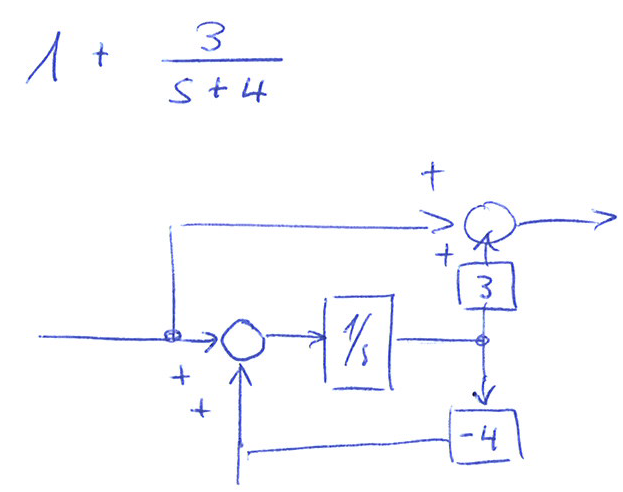
\includegraphics[width=5cm]{./images/implementierung2.png}
%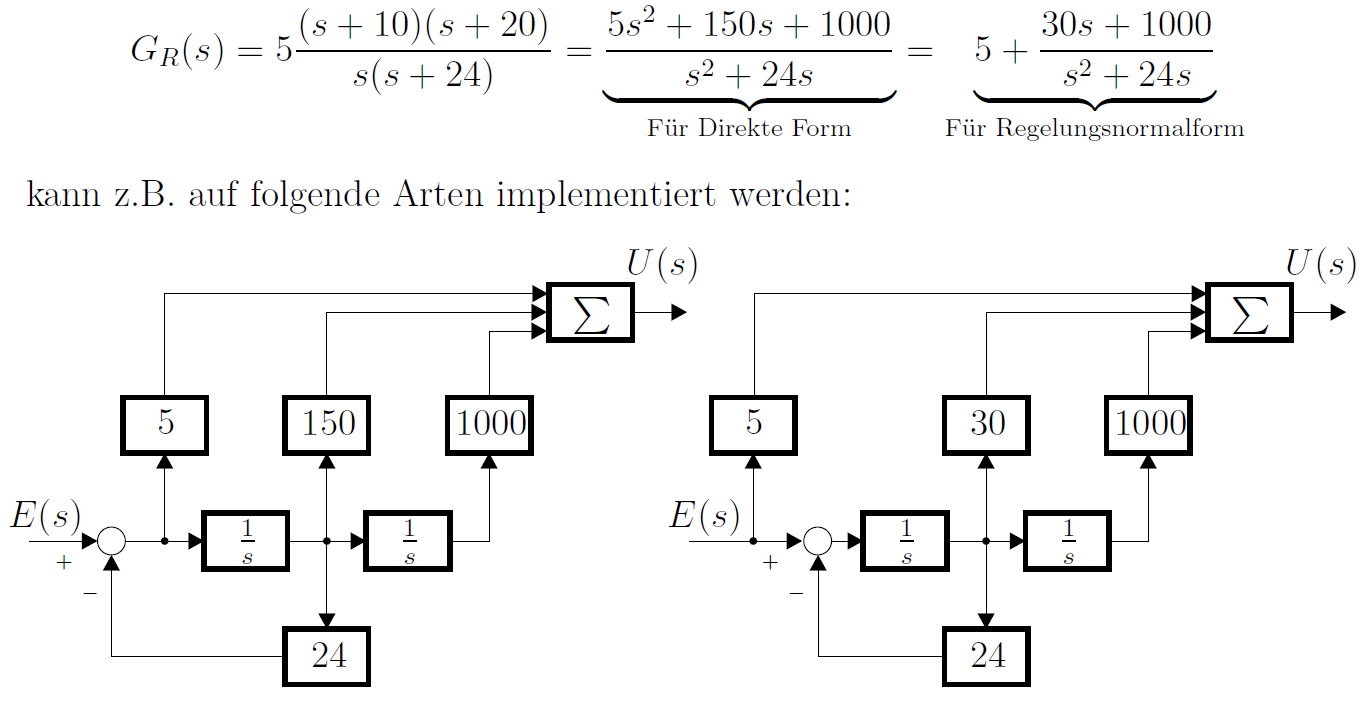
\includegraphics[width=10cm]{./images/implementierung.png}


\subsection{Direkte Form/ Direkte Form II}
\begin{center}
        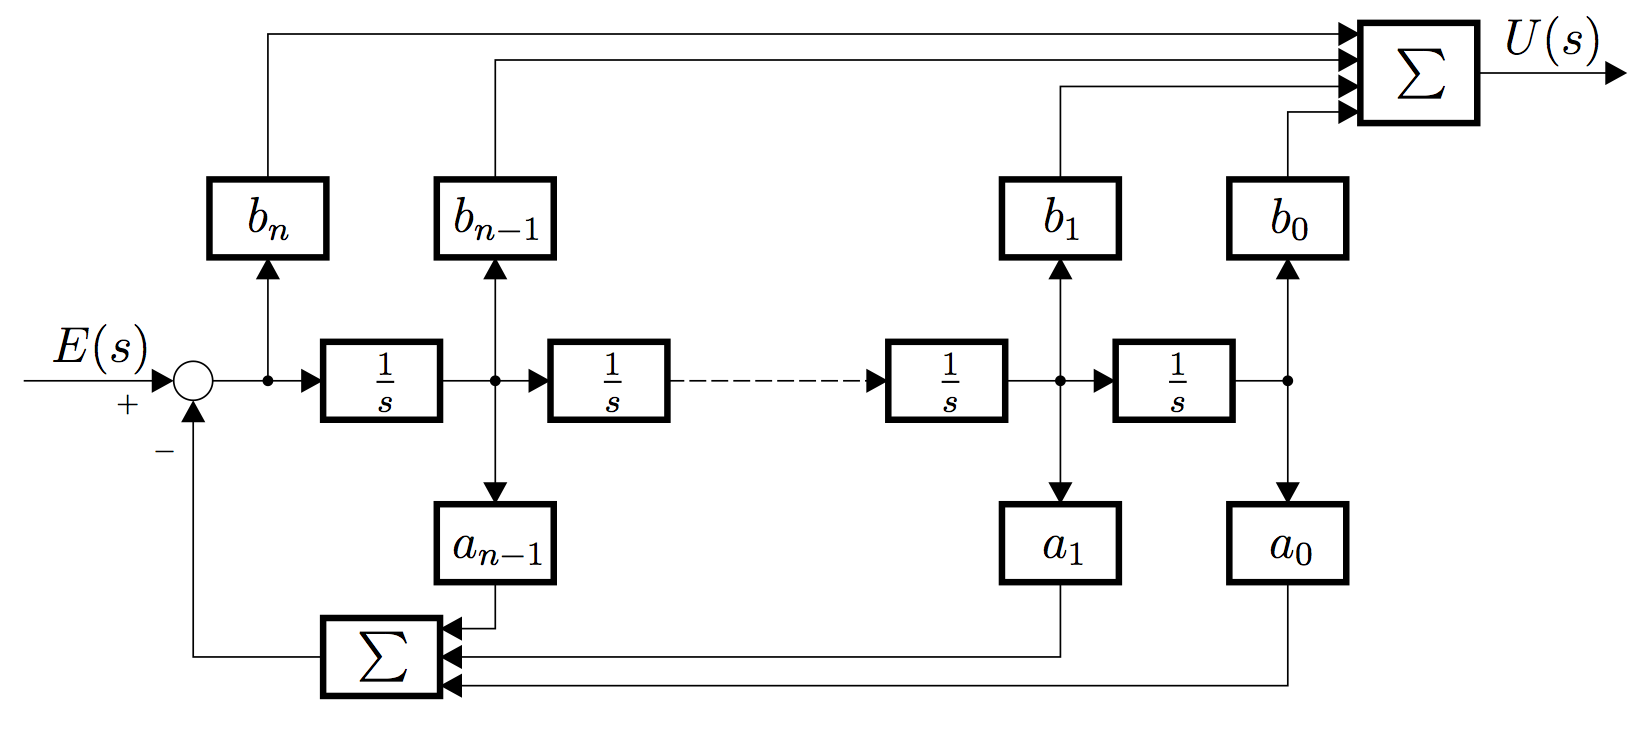
\includegraphics[width = 12cm]{./images/DirekteForm2}
\end{center}


\subsection{Transponierte direkte Form/ Direkte Form I}
\begin{center}
    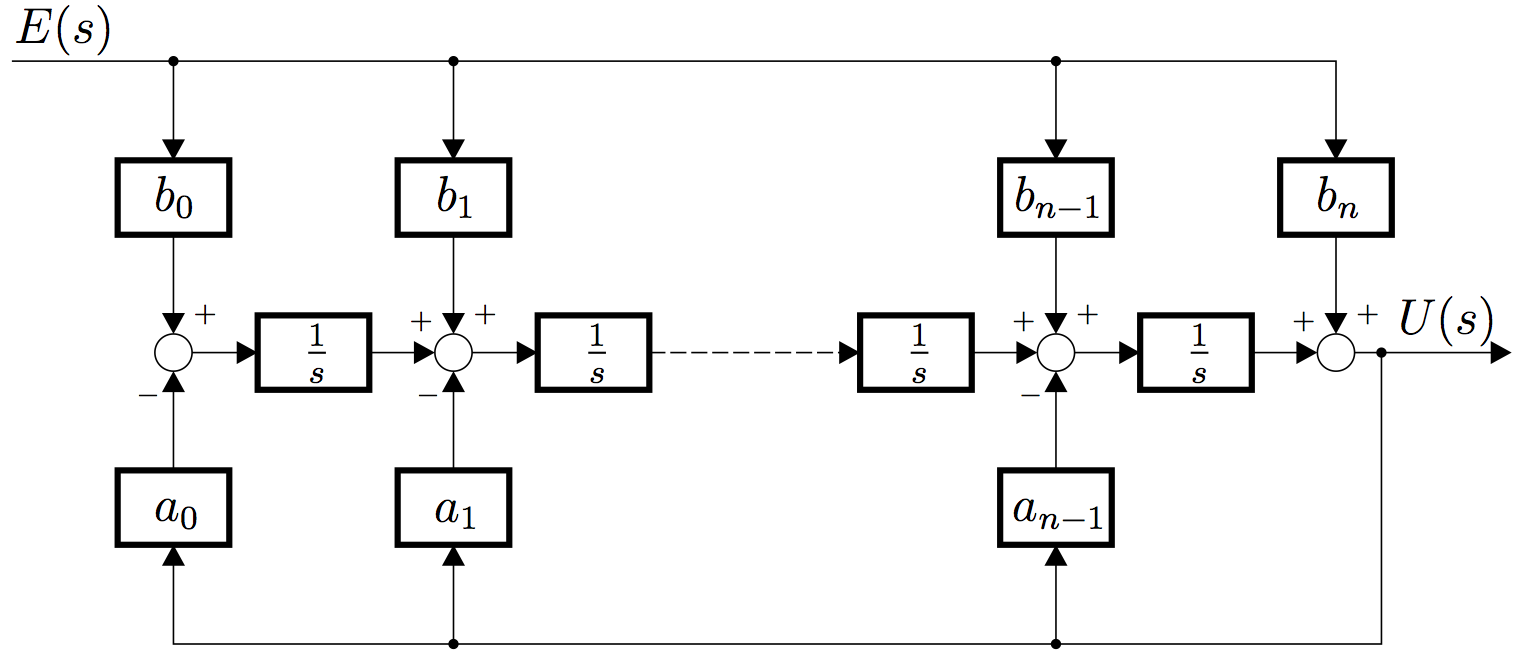
\includegraphics[width = 12cm]{./images/DirekteForm1}
\end{center}